\documentclass[11pt]{article}

\usepackage[preprint]{neurips_2025}
\usepackage[T1]{fontenc}
\usepackage{amsmath}
\usepackage{amssymb}
\usepackage{booktabs}
\usepackage{array}
\usepackage{siunitx}
\sisetup{table-number-alignment=center, table-format=2.2}
\usepackage{enumitem}
\usepackage{float}
\usepackage{graphicx}
\graphicspath{{./}{../../}}
\usepackage{hyperref}
\usepackage{xcolor}
\usepackage{caption}
\usepackage{tikz}
\usetikzlibrary{arrows.meta, shapes.geometric, positioning, fit, backgrounds}

\hypersetup{
  colorlinks=true,
  linkcolor=blue!50!black,
  citecolor=blue!50!black,
  urlcolor=blue!50!black
}

\captionsetup{
  font=small,
  labelfont=bf
}

\title{\textbf{Factor-Anchored Reinforcement Learning for Portfolio Risk Control}\\
\Large Evidence from Frozen-Bundle Evaluation under Timing and Cost Constraints}
\author{Ioan Hedea}
\date{}

\begin{document}
\maketitle

\begin{abstract}
This paper studies whether reinforcement learning is more useful in equity
trading as a control layer than as an end-to-end predictor. The evaluated setup
is a modular, factor-anchored pipeline in which finance-first alpha models feed
a constrained allocator, while RL modulates exposure, protection, and execution
under explicit timing and transaction-cost assumptions. Rather than relying on a
best-case exploratory run, the paper ties its claims to a frozen archived
bundle spanning April 2013 to March 2026. In the main archived split, the full
pipeline reduces maximum drawdown relative to SPY by 9.8 percentage points
($-24.0\%$ versus $-33.7\%$), but it trails SPY on annualized return
(13.0\% versus 15.3\%) and Sharpe (0.53 versus 0.58). The factor-only
benchmark and the strongest rule-based overlays remain materially stronger on
return- and Sharpe-based comparisons, while differences versus end-to-end PPO
are mixed and statistically inconclusive. The supported conclusion is therefore
narrower still: in this archived bundle, RL is best viewed as an interpretable
risk-shaping overlay rather than as a source of top-line performance or a clear
win over end-to-end PPO.
\end{abstract}

\medskip
\noindent\textbf{Keywords:} quantitative trading, reinforcement learning, factor investing, statistical arbitrage, regime detection, risk management, backtesting

\section{Introduction}

Many quantitative trading systems are built from a collection of specialized
modules rather than from a single monolithic predictor. Cross-sectional factors,
relative-value signals, volatility models, and regime filters often contribute
distinct pieces of information about expected return and risk. Reinforcement
learning (RL), by contrast, is most compelling when the task is inherently
sequential: choosing when to increase risk, when to hedge, and how to adapt
execution to changing conditions \cite{sutton2018,almgren2000}.

This project adopts exactly that separation of responsibilities. The alpha layer
is intentionally finance-first. It draws on ideas from factor investing
\cite{fama1993,jegadeesh1993}, cointegration-based statistical arbitrage
\cite{engle1987}, conditional volatility modeling \cite{engle1982,bollerslev1986},
and regime detection \cite{hamilton1989}. The RL layer does not attempt to
discover alpha from scratch. Instead, it treats alpha as an input and learns how
aggressively to express it under different risk and market states.

The present implementation contributes five practical elements to the evaluation
setup.
\begin{enumerate}[leftmargin=1.5em, itemsep=2pt, topsep=4pt]
\item A modular code architecture that cleanly separates data, alpha, control,
      backtesting, and visualization concerns.
\item A factor-anchored portfolio construction policy in which RL primarily
      controls exposure and active overlay size rather than acting as a second
      stock selector.
\item A constrained optimization layer between alpha and RL that turns signal
      forecasts into a capped, turnover-aware, and group-aware target book.
\item An IV-aware synthetic option-overlay sleeve and transaction-cost model
      that make the backtest more realistic while remaining implementable with
      public daily data.
\item A research evaluation workflow including ablations, rolling windows,
      sensitivity tests, and regime-conditioned policy summaries.
\end{enumerate}

\subsection{Research Questions}

The current version of the report is organized around three explicit research
questions.
\begin{enumerate}[leftmargin=1.5em, itemsep=2pt, topsep=4pt]
\item \textbf{RQ1: Controller vs.\ end-to-end RL.} Is reinforcement learning
      more effective as a modular control layer over financially grounded alpha
      models than as an end-to-end trading agent?
\item \textbf{RQ2: Value over simple rules.} Does the RL control layer add
      measurable value beyond rule-based heuristics such as volatility targeting
      and drawdown-based deleveraging?
\item \textbf{RQ3: Component attribution.} Which part of the control layer,
      exposure modulation, dynamic hedging, or their joint operation, is the
      primary driver of the observed risk transformation?
\end{enumerate}

\subsection*{Beyond the Present Manuscript}
\textit{A natural next step, not evaluated in the present manuscript, concerns
hedge realism: whether implied-volatility-conditioned, option-style overlays
such as protective puts, collars, and put spreads improve the downside sleeve
beyond the current stylized convex hedge approximation.}

From a research perspective, this framing matters because it narrows the gap
between a teaching prototype and a system that can be discussed in the language
of quantitative portfolio construction. The objective is not to claim that the
pipeline is production-ready. Rather, it is to assemble a well-motivated stack
in which each modeling choice has a clear financial role and where performance
can be decomposed into alpha generation, risk transformation, and control.

The central defended statement of the paper is therefore sharper than ``the
system works.'' \emph{A factor-anchored RL control layer, evaluated under
explicit cost and timing assumptions, can serve as a disciplined downside-
shaping overlay relative to passive exposure while remaining more interpretable
than an end-to-end policy.} \emph{The paper does not claim that this RL layer
surpasses SPY, PPO, or the strongest finance-first and rule-based baselines on
return- and Sharpe-based comparisons in the archived bundle.}
That narrower empirical outcome is still useful, because it helps separate
where RL contributes to risk transformation from where simpler finance-first
mechanisms remain stronger. The rest of the paper is organized to test that
claim rather than merely to catalogue modules.

\section{Related Literature and Design Motivation}

The report is not meant to claim novelty in any individual modeling choice.
Instead, it builds a coherent pipeline from well-established ingredients.

\textbf{Factor investing.} The cross-sectional component is aligned with the idea
that common risk factors help explain returns \cite{fama1993}. Momentum is
motivated by the medium-horizon continuation evidence of Jegadeesh and Titman
\cite{jegadeesh1993}, while quality and low-volatility proxies are included to
stabilize the cross-section.

\textbf{Statistical arbitrage.} The pairs sleeve follows the classical
cointegration logic of Engle and Granger \cite{engle1987}: if a spread is mean
reverting around an equilibrium relation, deviations from that equilibrium may
carry predictive content.

\textbf{Volatility and regimes.} Conditional heteroskedasticity motivates the
GARCH sleeve \cite{engle1982,bollerslev1986}, while the market-regime component
uses a two-state hidden Markov model in the spirit of Hamilton \cite{hamilton1989}.

\textbf{Reinforcement learning.} RL is used as a controller rather than a raw
alpha generator. This follows the practical observation that in finance, RL is
often most useful for allocation, inventory, and execution decisions rather than
for replacing domain-specific signal construction \cite{sutton2018,almgren2000}.
This role assignment is also motivated by the low signal-to-noise ratio and
limited effective sample size typical of financial data, which make end-to-end
policy learning especially brittle.

\textbf{Rule-based risk management and controller baselines.} A key part of the
evaluation design is to compare the RL controller not only with passive
benchmarks but also with rule-based heuristics that a skeptical reader would
reasonably propose as simpler substitutes. In this project, the most important
examples are volatility targeting and drawdown-based deleveraging. These
baselines matter because they help distinguish ``RL adds value'' from ``any
reasonable overlay would have helped.''

\subsection{Recent Work on RL for Portfolio Management}

Recent work on RL in portfolio management and trading can be organized into four
overlapping strands.

\textbf{End-to-end policy learning.} Early and influential work uses RL to learn
trading or allocation policies directly from price histories and realized
rewards \cite{moody2001,deng2017,jiang2017,zhang2020,cong2021,pacheco2023}. The appeal of
this approach is conceptual elegance: the same learner is asked to extract
signal, size positions, and adapt sequentially. The difficulty is that
financial returns are noisy, nonstationary, and data-poor relative to many
other machine-learning domains. As a result, end-to-end RL systems can be
sample-inefficient, regime-sensitive, and hard to interpret when they fail
\cite{gu2020,kolm2019,jander2025}.

\textbf{Neural return forecasting with a separate optimizer.} A second line of
work uses deep or other machine-learning models to estimate returns, factors, or
pricing kernels, then hands those forecasts to a conventional optimizer
\cite{gu2020,chen2021,giglio2022}. This preserves more structure in the
allocation step than end-to-end RL, and often performs well empirically, but it
still concentrates modeling risk in a data-hungry prediction layer.

\textbf{RL for execution, hedging, and risk control.} A third strand applies RL
to narrower sequential tasks such as execution, hedging, and dynamic risk
management rather than to raw alpha discovery \cite{nevmyvaka2006,kolm2019hedge,
buehler2019,du2020}. This decomposition is closest to the present paper. The
core idea is that RL may be most useful where the problem is inherently
sequential and control-like, while alpha generation remains anchored to domain
models or explicit financial structure.

\textbf{Benchmarking and reproducibility.} More recent platform and survey work
has emphasized that RL in finance still suffers from weak evaluation discipline,
narrow datasets, and inconsistent reporting \cite{sun2023,jander2025}. That
critique directly motivates the frozen-bundle methodology used here. The paper
is not only a claim about architecture; it is also a claim about how such
architectures should be evaluated.

Table~\ref{tab:taxonomy} positions the present approach relative to these
broader families. The contribution is not a new RL algorithm. It is a
methodological proposal: if strong finance-first alpha already exists, RL should
be tested primarily as a controller layered on top of that alpha, then judged
against both simple rule-based overlays and end-to-end learned alternatives.

\begin{table}[H]
\centering
\scriptsize
\caption{Taxonomy of portfolio-management architectures.}
\label{tab:taxonomy}
\begin{tabular}{@{} >{\raggedright\arraybackslash}p{2.1cm}
                >{\raggedright\arraybackslash}p{2.1cm}
                >{\raggedright\arraybackslash}p{2.15cm}
                >{\raggedright\arraybackslash}p{1.45cm}
                >{\raggedright\arraybackslash}p{4.2cm} @{}}
\toprule
\textbf{Approach} & \textbf{Alpha source} & \textbf{Control logic} & \textbf{Interp.} & \textbf{Representative references} \\
\midrule
Classical factors & Hand-crafted financial signals & Fixed allocator or simple overlay rules & High & Fama--French style factor investing \cite{fama1993} \\
End-to-end RL & Learned from market histories & RL policy directly selects positions or weights & Low to medium & Direct trading and portfolio RL \cite{moody2001,jiang2017,zhang2020,cong2021} \\
Neural forecasting + optimizer & Neural or ML return forecasts & Separate optimizer translates forecasts into holdings & Medium & Asset-pricing and return-forecast models \cite{gu2020,chen2021,giglio2022} \\
\textbf{This paper} & \textbf{Finance-first alpha models} & \textbf{RL modulates exposure, hedging, and execution} & \textbf{High} & \textbf{Frozen-bundle control-layer evaluation} \\
\bottomrule
\end{tabular}
\end{table}

\subsection{Contribution Type}

The contribution is not novelty in any single alpha ingredient. The paper does
not claim a new factor model, a new GARCH variant, or a new hidden-state
estimator. Its contribution lies instead in three places. First, it proposes a
clear role assignment between alpha and control: financially grounded models
produce expected-return structure, while RL handles sequential exposure and
protection decisions. Second, it implements that role assignment in a modular
architecture with an explicit constrained allocator between alpha and control.
Third, it pairs the architecture with an evaluation workflow designed to test
that claim via ablations, timing-discipline checks, robustness slices, and
regime-conditional policy analysis.
The contribution is therefore chiefly methodological: the paper proposes and
tests a disciplined way to evaluate RL as a control layer rather than as a
monolithic trading policy.

\section{System Architecture}

The pipeline is organized as a linear sequence of stages, illustrated in
Figure~\ref{fig:architecture}. Each stage has a clearly delimited responsibility:
upstream stages produce signals and risk features, the control layer translates
these into portfolio decisions, and the backtest layer evaluates realized
outcomes.

\begin{figure}[H]
\centering
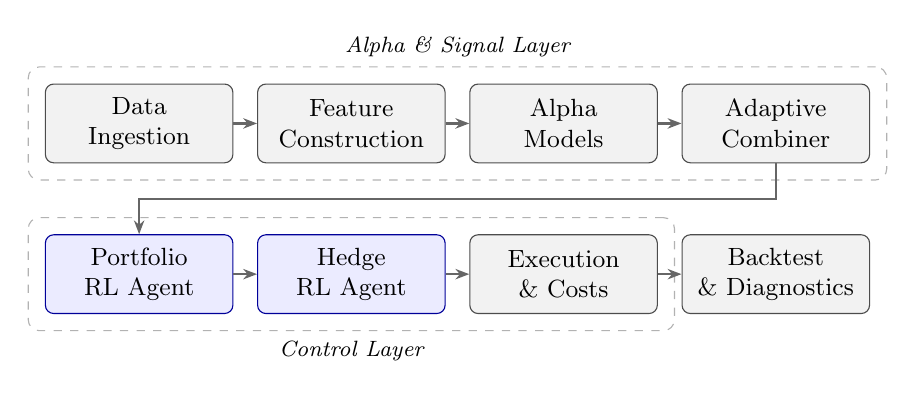
\begin{tikzpicture}[
  node distance = 0.45cm and 0.30cm,
  box/.style = {
    rectangle, rounded corners=3pt,
    draw=black!70, fill=gray!10,
    text width=2.1cm, align=center,
    font=\small, minimum height=1.0cm,
    inner sep=4pt
  },
  rlbox/.style = {
    rectangle, rounded corners=3pt,
    draw=blue!60!black, fill=blue!8,
    text width=2.1cm, align=center,
    font=\small, minimum height=1.0cm,
    inner sep=4pt
  },
  arr/.style = {-{Stealth[length=5pt]}, thick, black!60},
  groupbox/.style = {
    draw=black!30, dashed, rounded corners=4pt,
    fill=none, inner sep=6pt
  }
]

% Row 1: Data → Features → Alpha Models → Adaptive Combiner
\node[box] (data)    {Data\\Ingestion};
\node[box, right=of data]    (feat)    {Feature\\Construction};
\node[box, right=of feat]    (alpha)   {Alpha\\Models};
\node[box, right=of alpha]   (comb)    {Adaptive\\Combiner};

% Row 2: Portfolio RL → Hedge/Cash → Backtest
\node[rlbox, below=0.9cm of data]  (portrl)  {Portfolio\\RL Agent};
\node[rlbox, right=of portrl]      (hedgerl) {Hedge\\RL Agent};
\node[box,   right=of hedgerl]     (exec)    {Execution\\\& Costs};
\node[box,   right=of exec]        (bt)      {Backtest\\\& Diagnostics};

% Row 1 arrows
\draw[arr] (data)  -- (feat);
\draw[arr] (feat)  -- (alpha);
\draw[arr] (alpha) -- (comb);

% Combiner down to portfolio RL
\draw[arr] (comb.south) -- ++(0,-0.45) -| (portrl.north);

% Row 2 arrows
\draw[arr] (portrl)  -- (hedgerl);
\draw[arr] (hedgerl) -- (exec);
\draw[arr] (exec)    -- (bt);

% Labels
\begin{scope}[on background layer]
  \node[groupbox, fit=(data)(feat)(alpha)(comb),
        label={[font=\footnotesize\itshape]above:Alpha \& Signal Layer}] {};
  \node[groupbox, fit=(portrl)(hedgerl)(exec),
        label={[font=\footnotesize\itshape]below:Control Layer}] {};
\end{scope}
\end{tikzpicture}
\caption{High-level architecture of the quantitative trading pipeline. The alpha
and signal layer (top) produces expected-return scores and risk features; the
control layer (bottom) translates these into portfolio weights, hedge intensity,
and cash allocation before evaluation in the backtest engine.}
\label{fig:architecture}
\end{figure}

\subsection{Software Structure}

\begin{table}[H]
\centering
\caption{Module-level decomposition of the \texttt{quant\_stack} package.}
\begin{tabular}{@{} l p{9.5cm} @{}}
\toprule
\textbf{Module} & \textbf{Responsibility} \\
\midrule
\texttt{config.py}   & Universe definition, global constants, and external series identifiers \\
\texttt{data.py}     & Market price/volume ingestion, macro series (FRED / BLS fallback), and SEC company facts \\
\texttt{alpha.py}    & Cross-sectional factors, pairs cointegration, GARCH volatility, HMM regime, LSTM forecast, and adaptive signal combination \\
\texttt{rl.py}       & Portfolio construction agent, execution controller, and dynamic hedging agent \\
\texttt{pipeline.py} & Walk-forward backtest orchestration and online RL update loop \\
\texttt{evaluation.py} & Ablation, rolling-window robustness, sensitivity analysis, and research artifact export \\
\texttt{plots.py}    & Equity-curve, drawdown, RL behavior, and alpha-model diagnostic figures \\
\texttt{main.py}     & CLI entry point and compatibility wrapper \\
\bottomrule
\end{tabular}
\end{table}

This decomposition is important for research reproducibility. It keeps the
external command stable while turning the internals into separately testable
components.

\section{Data and Feature Construction}

\subsection{Universe}

The archived research bundle uses the expanded universe rather than the smaller
development basket. It contains 76 traded assets spread across technology,
financials, healthcare, consumer staples, energy, industrials, materials, real
estate, utilities, communications, and consumer discretionary, together with
three diversifiers: GLD, TLT, and VNQ. SPY serves as the passive equity
benchmark throughout.

\subsection{Data Sources}

The pipeline supports both a free baseline configuration and a richer research
configuration. Daily prices and volumes are sourced via \texttt{yfinance}. When a
\texttt{FRED\_API\_KEY} is available, macro data are drawn directly from FRED; in
its absence, the system falls back to BLS and U.S.\ Treasury Fiscal Data. SEC
company facts are incorporated when \texttt{SEC\_USER\_AGENT} is set, enabling a
light fundamentals layer without requiring a proprietary data subscription.

\subsection{Macro Regime Inputs}

When available, the macro sleeve includes rates and labor-market variables such
as the 10-year yield, 2-year yield, federal funds rate, unemployment rate, and
term spread. The updated research design also incorporates stress-sensitive FRED
series including the VIX, the ICE BofA high-yield option-adjusted spread, and a
dollar-index proxy. These variables do not form a standalone alpha book.
Instead, they help create a macro regime belief that is blended with the HMM
regime estimate and provide additional context for risk-off states.

\subsection{Uncertainty and Disagreement Features}

One of the most distinctive methodological additions is that the controller is
no longer conditioned only on point estimates. The updated state construction
also tracks uncertainty proxies derived from the alpha and regime stack. The
main examples are alpha-sleeve dispersion, regime-belief entropy, and rolling
instability in recent information coefficients. Intuitively, these features
measure three different kinds of uncertainty: disagreement across signals,
ambiguity in the inferred market state, and instability in the recent mapping
from scores to realized returns.

This matters because a sequential controller should not react the same way when
the alpha opportunity looks strong and coherent as when the same opportunity is
accompanied by high model disagreement or unstable recent signal quality. In
that sense, the control layer is not just regime-aware; it is also
uncertainty-aware.

\subsection{Information-Timing Contract}

One of the most important research upgrades in the current version is that the
pipeline now makes its feature-availability assumptions explicit. Macro inputs
are shifted forward by a configurable number of trading days before they are
allowed into the backtest. This is still weaker than a true real-time vintage
database, because it does not model revisions, but it is materially stronger
than using the final macro history with no delay assumption at all.

Fundamental inputs are handled more conservatively. The SEC quality signal is
still a static cross-sectional research prior rather than a fully point-in-time
fundamentals panel. For that reason the research engine now supports a strict
timing mode in which the SEC quality sleeve is disabled and macro inputs are
forced to use the largest configured lag. The point of this design is not to
pretend that point-in-time fundamentals are already solved, but rather to make
the timing caveat measurable and visible in the evaluation workflow.

\section{Methodology}

\subsection{Problem Formulation}

Let $r_{t+1} \in \mathbb{R}^N$ denote next-period asset returns for a universe of
$N$ tradable assets. At time $t$, the system observes a feature state
$x_t \in \mathcal{X}$ constructed from cross-sectional factor values,
relative-value spreads, volatility forecasts, regime beliefs, and macro inputs.
The alpha layer maps these features into an expected-return score vector
$\alpha_t \in \mathbb{R}^N$ and a confidence vector $c_t \in \mathbb{R}^N$.

The control layer then chooses a portfolio allocation $w_t$, a cash allocation,
and a hedge intensity $h_t$. The one-step portfolio objective is not written as
a pure return maximization problem. Instead, it is implicitly multi-objective:
maximize long-run wealth while limiting drawdown, volatility, and unnecessary
turnover. This is the reason the project separates alpha estimation from control:
the two tasks operate on different time scales and carry different inductive
biases.
Importantly, the RL layer does not forecast $r_{t+1}$ directly; it maps a state
summarizing alpha quality and risk conditions into exposure, overlay, and
protection decisions.

\subsection{Cross-Sectional Factor Model}

The factor sleeve combines four z-scored components: momentum, a value proxy, a
quality proxy, and a low-volatility tilt. Letting $m_i$, $v_i$, $q_i$, and
$\ell_i$ denote the standardized scores for asset
$i$, the composite factor score is
\[
f_i = 0.30 m_i + 0.25 v_i + 0.25 q_i + 0.20 \ell_i.
\]

This choice reflects a balanced, multi-style factor book rather than a single
directional bet.

\subsection{Pairs Trading}

For candidate pairs, a hedge ratio $\beta$ is estimated by OLS and the spread
\[
s_t = P^{(1)}_t - \beta P^{(2)}_t
\]
is normalized into a z-score
\[
z_t = \frac{s_t - \mu_s}{\sigma_s + \varepsilon}.
\]
Large positive z-scores correspond to short-spread trades and large negative
z-scores correspond to long-spread trades.

\subsection{Volatility and Regime Models}

Each name receives a GARCH(1,1) forecast
\[
\sigma_t^2 = \omega + \alpha_1 \epsilon_{t-1}^2 + \beta_1 \sigma_{t-1}^2,
\]
where $\omega > 0$, $\alpha_1 \geq 0$, and $\beta_1 \geq 0$ are the intercept,
ARCH, and GARCH coefficients respectively. This conditional variance estimate
is used for confidence scaling and risk awareness. Separately, a two-state
HMM produces a bull-versus-bear regime belief. The final regime signal is
\[
\text{RegimeBelief}_t =
0.75 \cdot \text{HMMBelief}_t +
0.25 \cdot \text{MacroBelief}_t.
\]

\subsection{Adaptive Alpha Combination}

Let $s^{(k)}_{i,t}$ denote the signal from source $k$ for asset $i$ at time $t$.
The expected return score is formed as
\[
\alpha_{i,t} = \sum_k w^{(k)}_t s^{(k)}_{i,t},
\]
where the source weights $w^{(k)}_t$ adapt over time based on recent realized
signal quality. In the implementation, this is proxied by recent Spearman
information coefficients between source scores and realized returns.

This adaptive weighting is important because the constituent alpha sleeves are
not equally informative across all market states. Pairs signals can be weak in
strongly trending markets, deep nonlinear forecasts can degrade when regime
structure shifts, and factor signals can vary in efficacy depending on the
dispersion of the cross-section. The adaptive combiner therefore behaves like a
simple online model-selection layer.

\subsection{Portfolio Construction RL}

The portfolio RL state summarizes the current cross-sectional alpha
opportunity, recent realized portfolio volatility, the prevailing regime
belief, and an uncertainty score built from alpha dispersion, regime entropy,
and recent IC instability. Crucially, the policy is \emph{factor-anchored}. The
target book is
\[
w_t^{\text{target}} =
0.90\,w_t^{\text{factor}} +
0.10\,w_t^{\text{stabilizer}},
\]
where the stabilizer is a long-only minimum-variance-style portfolio estimated
from a Ledoit--Wolf shrinkage covariance matrix.

If the RL agent chooses invested fraction $b_t$ and active overlay size $\tau_t$,
the final invested portfolio is approximately
\[
w_t =
b_t \left[(1-\tau_t)w_t^{\text{target}} + \tau_t w_t^{\text{satellite}}\right].
\]
The satellite sleeve is not a fully independent book; it tilts the factor target
toward the strongest alpha names. This keeps the full pipeline close to the
working factor engine while still letting RL modulate aggressiveness.

Between the alpha combiner and the RL policy, the code now inserts a constrained
intermediate allocator. The optimizer is long-only and solves a small
regularized problem of the form
\[
\min_w \quad
\lambda_{\mathrm{risk}} w^\top \Sigma_t w
- \lambda_{\alpha}\alpha_t^\top w
+ \lambda_{\mathrm{anchor}}\lVert w - w_t^{\mathrm{target}} \rVert_2^2
+ \lambda_{\mathrm{turn}}\lVert w - w_{t-1} \rVert_2^2
\]
subject to $w_i \ge 0$, $\sum_i w_i = 1$, per-asset caps, and simple group
concentration limits. This layer is architecturally important because it makes
the separation of concerns sharper: alpha expresses expected return, the
optimizer expresses institutional portfolio constraints, and RL governs when to
lean into or away from that target book.
This intermediate layer is not only an architectural convenience; it reflects
the practical fact that many real portfolio systems mediate between forecast
signals and final positions through a constrained allocator.

\subsection{Reward Design}

The portfolio RL update uses a differential Sharpe-style reward based on the
realized portfolio return relative to a recent rolling distribution of returns.
In compact form,
\[
R_t^{\mathrm{portfolio}}
= \frac{r_t - \hat{\mu}_t}{\hat{\sigma}_t + \varepsilon},
\]
where $\hat{\mu}_t$ and $\hat{\sigma}_t$ are running estimates of recent mean
return and volatility. This means the agent is not rewarded solely for taking
more risk in absolute terms; it is rewarded for improving return relative to
the recent volatility environment.

The hedge agent uses an asymmetric realized-return reward in which losses are
penalized more heavily than gains are rewarded. A stylized form is
\[
R_t^{\mathrm{hedge}}
= r_t \mathbf{1}(r_t \ge 0)
 + \lambda_{\mathrm{loss}} r_t \mathbf{1}(r_t < 0),
\qquad \lambda_{\mathrm{loss}} > 1.
\]
That asymmetry is a deliberate design choice: it pushes the hedge layer toward
preserving capital in stress rather than maximizing average carry.

The research runner is now also designed to support reward-function ablations.
In addition to the default differential-Sharpe-style objective, the evaluation
protocol can compare raw-return and Sortino-style reward formulations. This
matters because reward design is one of the least observable but most important
degrees of freedom in RL-for-finance systems.
Because reward specification changes the controller's operating point, it should
be treated as a methodological degree of freedom rather than as a neutral
implementation detail.

\subsection{No-Trade Band and Hedging}

To reduce turnover drag, a rebalance band suppresses small changes in target
weights. When only part of the portfolio is changed, the active weights are
rescaled to preserve the desired capital budget.

The hedging RL layer observes drawdown, volatility regime, recent momentum, and
IV-aware option-overlay features. In the archived experiment reported here, it
chooses both one of four hedge intensities and one proxy overlay type among a
protective put, a collar, and a put spread. The total one-period return can be
written schematically as
\[
r_t^{	ext{total}} =
r_t^{	ext{risky}}(1-\phi h_t) + r_t^{	ext{cash}} + r_t^{	ext{hedge}},
\]
where $h_t$ is the hedge fraction and $r_t^{	ext{hedge}}$ includes carry,
option-style payoff asymmetry, and a state-dependent protection term.

This is more realistic than the earlier convex-loss proxy, but it is still not a
market-priced options backtest. The overlay payoffs are generated from public
IV and market-stress proxies rather than live option-chain quotes. The reported
hedge sleeve should therefore be interpreted as a synthetic option-style overlay
rather than as a fully market-consistent derivatives implementation.

\subsection{Transaction Costs and Execution Realism}

The backtest now includes a three-part execution-cost approximation. For each
rebalance, the strategy pays a fixed basis-point fee on turnover, an additional
penalty proportional to turnover times realized volatility, and a size penalty
linked to the largest one-name weight change. In symbols,
\[
\mathrm{TC}_t
= c_0 \cdot \mathrm{turnover}_t
+ c_1 \cdot \mathrm{turnover}_t \cdot \hat{\sigma}_t
+ c_2 \cdot \max_i |\Delta w_{i,t}|.
\]
This is not a full execution simulator, but it pushes the daily allocator away
from unrealistic churn and makes the rebalance band economically meaningful
rather than purely cosmetic.

\section{Experimental Design}

The archived bundle used in the paper contains approximately 3{,}270 daily
observations from early April 2013 through late March 2026. The reported main
split trains the upstream statistical components on the initial segment through
September 25, 2019 and then evaluates the walk-forward controller from
September 25, 2019 to March 27, 2026. The manuscript is tied to this frozen
archived bundle, saved on March 28, 2026 as the latest complete research run
for the expanded-universe configuration, even though the live codebase may
already contain extensions not exercised by the reported evidence. This does
not eliminate prior exploratory iteration, but it does make the reported
bundle explicit and reproducible. Within the archived suite itself, action
ladders, optimizer settings, reward choices, and comparison baselines are held
fixed across ablations, split-fraction tests, and rolling-window robustness
slices.

Within that archived run, the LSTM sleeve is first trained on the initial
window, after which the full pipeline is rolled forward one trading day at a
time with the configuration held fixed during evaluation.

At each date, the pipeline executes the following sequence. First, factor,
pairs, GARCH, HMM, macro, and LSTM features are generated from the available
data. These are combined into expected-return scores and confidence levels via
the adaptive combiner. The portfolio RL agent then selects an exposure bucket
and overlay size, after which the hedge agent chooses both a hedge intensity and
a proxy option-overlay type. Transaction costs, cash carry, and hedge payoffs
are applied to arrive at the realized portfolio return, which is finally used
to update both RL value tables before advancing to the next trading day.

The comparison set now goes beyond passive and naive portfolio baselines. In
addition to SPY buy-and-hold and the factor-only benchmark, the research
protocol includes a volatility-targeting overlay on the factor book, a
drawdown-based deleveraging rule, and an end-to-end PPO baseline that receives
the same broad information set as the modular architecture. These additions are
essential for the paper's research questions because they test whether RL adds
value over simple heuristics and whether modular control is preferable to a
monolithic learning policy.

\subsection{Benchmark Logic}

The benchmark set is chosen to isolate different sources of value. SPY measures
whether the pipeline adds value relative to standard passive equity exposure.
The factor-only benchmark isolates the pure alpha layer without any RL overlay.
Because the archived bundle already uses a broad 76-asset universe, this factor
benchmark is also informative about what the diversified opportunity set can do
without RL control. Comparing the full pipeline against the factor-only
benchmark is particularly important because it reveals whether RL is adding
value as a controller or merely acting as a drag on a strong signal engine.

The newer comparison baselines sharpen that logic further. The volatility
targeting baseline asks whether most of the observed improvement can be matched
by simple inverse-vol scaling. The drawdown-based deleveraging baseline asks
whether a threshold rule can replicate the protection sleeve's effect. The
end-to-end PPO baseline addresses the paper's most distinctive architectural
question: if one hands the same state information to a monolithic policy, does
it outperform a hybrid design in which finance-specific modules produce the
target book and RL only controls how aggressively to express it? These
baselines are deliberately strong because they represent the kinds of simple
overlays a practitioner would try before accepting the complexity of RL.

\section{Evaluation Metrics}

The reporting suite includes annualized return, annualized volatility, Sharpe
ratio, Sortino ratio, maximum drawdown, Calmar ratio, and return-distribution
diagnostics including a daily 5\% Value-at-Risk estimate.

If $\{r_t\}_{t=1}^T$ denotes daily portfolio returns and $r_f$ is the annual
risk-free rate, then the annualized Sharpe ratio is
\[
\text{Sharpe} = \frac{252 \, \bar{r} - r_f}{\sqrt{252}\,\hat{\sigma}(r) + \varepsilon}.
\]
The Sortino ratio replaces total volatility with downside volatility, while the
Calmar ratio scales annualized return by the magnitude of maximum drawdown. Each
metric emphasizes a different aspect of the return distribution, which matters in
this project because the pipeline is explicitly designed to reshape tail risk,
not merely to maximize mean return.
Table~\ref{tab:metrics} focuses on the primary comparison metrics used in the
main strategy table: return, volatility, Sharpe, maximum drawdown, and Calmar.
Sortino and Value-at-Risk are retained as secondary diagnostics in the text,
reward-ablation evidence, and archived research artifacts.

In addition, the research runner emits regime-conditional summaries of
portfolio action, hedge ratio, cash weight, turnover, transaction-cost drag, and
realized returns. These diagnostics help evaluate whether the controller
behaves differently in bullish, neutral, and bearish states in a way that is
consistent with the design intent of the policy.

For statistical reliability, the updated evaluation design also includes
block-bootstrap confidence intervals on daily-return paths. The motivation is to
preserve some of the short-horizon dependence structure in returns while still
providing uncertainty bands for quantities such as annualized return, Sharpe,
Calmar, and pairwise performance differences versus benchmark strategies.

\section{Results}

This section moves from the main walk-forward evidence to ablation, comparisons
against rule-based overlays and end-to-end PPO, rolling robustness slices,
blocked time-series cross-validation, and regime-conditioned behavior. The
organizing question throughout is whether the data support the narrower claim
that RL helps more as a controller than as a predictor.

\subsection{Main Result}

The archived research run used for the paper's main evidence evaluates the
walk-forward controller from September 25, 2019 to March 27, 2026. The summary
metrics are shown in Table~\ref{tab:metrics}. This is still only one realized
path, but it is the same frozen checkpoint that also feeds the ablation,
robustness, and significance artifacts discussed in the remainder of the paper.

\begin{table}[t]
\centering
\caption{Performance summary on the walk-forward test window
  (25 Sep 2019 -- 27 Mar 2026). Annualized figures. Max DD denotes maximum
  peak-to-trough drawdown; Calmar is annualized return divided by $|\text{Max DD}|$.}
\label{tab:metrics}
\begin{tabular}{@{} l r r r r r @{}}
\toprule
\textbf{Strategy} & \textbf{Return} & \textbf{Volatility} & \textbf{Sharpe} & \textbf{Max DD} & \textbf{Calmar} \\
\midrule
Full pipeline         & 13.0\% & 17.8\% & 0.53 & $-$24.0\% & 0.54 \\
SPY                   & 15.3\% & 20.2\% & 0.58 & $-$33.7\% & 0.45 \\
Factor-only benchmark & 26.6\% & 23.0\% & 1.00 & $-$33.8\% & 0.79 \\
Vol-target            & 16.3\% & 14.3\% & 0.89 & $-$20.6\% & 0.79 \\
DD-Delever            & 19.3\% & 17.1\% & 0.92 & $-$21.4\% & 0.90 \\
E2E RL (PPO)          & 8.7\%  & 9.2\%  & 0.56 & $-$15.5\% & 0.56 \\
\bottomrule
\end{tabular}
\end{table}

The main result is now more clearly mixed than favorable. That shift matters,
because it forces the paper to defend only the claims that survive the expanded
universe and longer sample.

Relative to SPY, the full pipeline is weaker on annualized return, 13.0\%
versus 15.3\%, and slightly weaker on Sharpe, 0.53 versus 0.58. Its favorable
result is narrower: maximum drawdown improves by about 9.8 percentage points,
from $-$33.7\% for SPY to $-$24.0\% for the full pipeline, and Calmar improves
modestly from 0.45 to 0.54. The passive-benchmark comparison therefore supports
downside reshaping, but not broad outperformance.

Relative to the factor-only benchmark, the conclusion is decisively negative.
The full pipeline trails by roughly 13.6 percentage points of annualized return
and by about 0.47 of Sharpe. The factor core remains the strongest pure alpha
expression in the archived bundle.

Relative to the strongest rule-based overlays, the result is again negative.
Volatility targeting and drawdown-based deleveraging both beat the full
pipeline on return and Sharpe, and they do so with drawdowns that are shallower
than, or at least comparable to, the RL stack.

Relative to the end-to-end PPO baseline, the result is mixed rather than
favorable. The full pipeline earns a higher annualized return, 13.0\% versus
8.7\%, but slightly lower Sharpe, 0.53 versus 0.56, and materially worse
maximum drawdown, $-$24.0\% versus $-$15.5\%. The main table therefore does
not provide a clean modular-over-PPO win on point estimates.

\noindent\textit{Implication for RQ1 and RQ2.} The main table is mostly
unfavorable for the RL layer. Drawdown improvement relative to SPY survives,
but neither superiority to strong rule-based overlays nor a clear advantage
over end-to-end PPO is supported.

\IfFileExists{../../results/20260328_experiments/pipeline_research_eval.png}{
\begin{figure}[t]
\centering
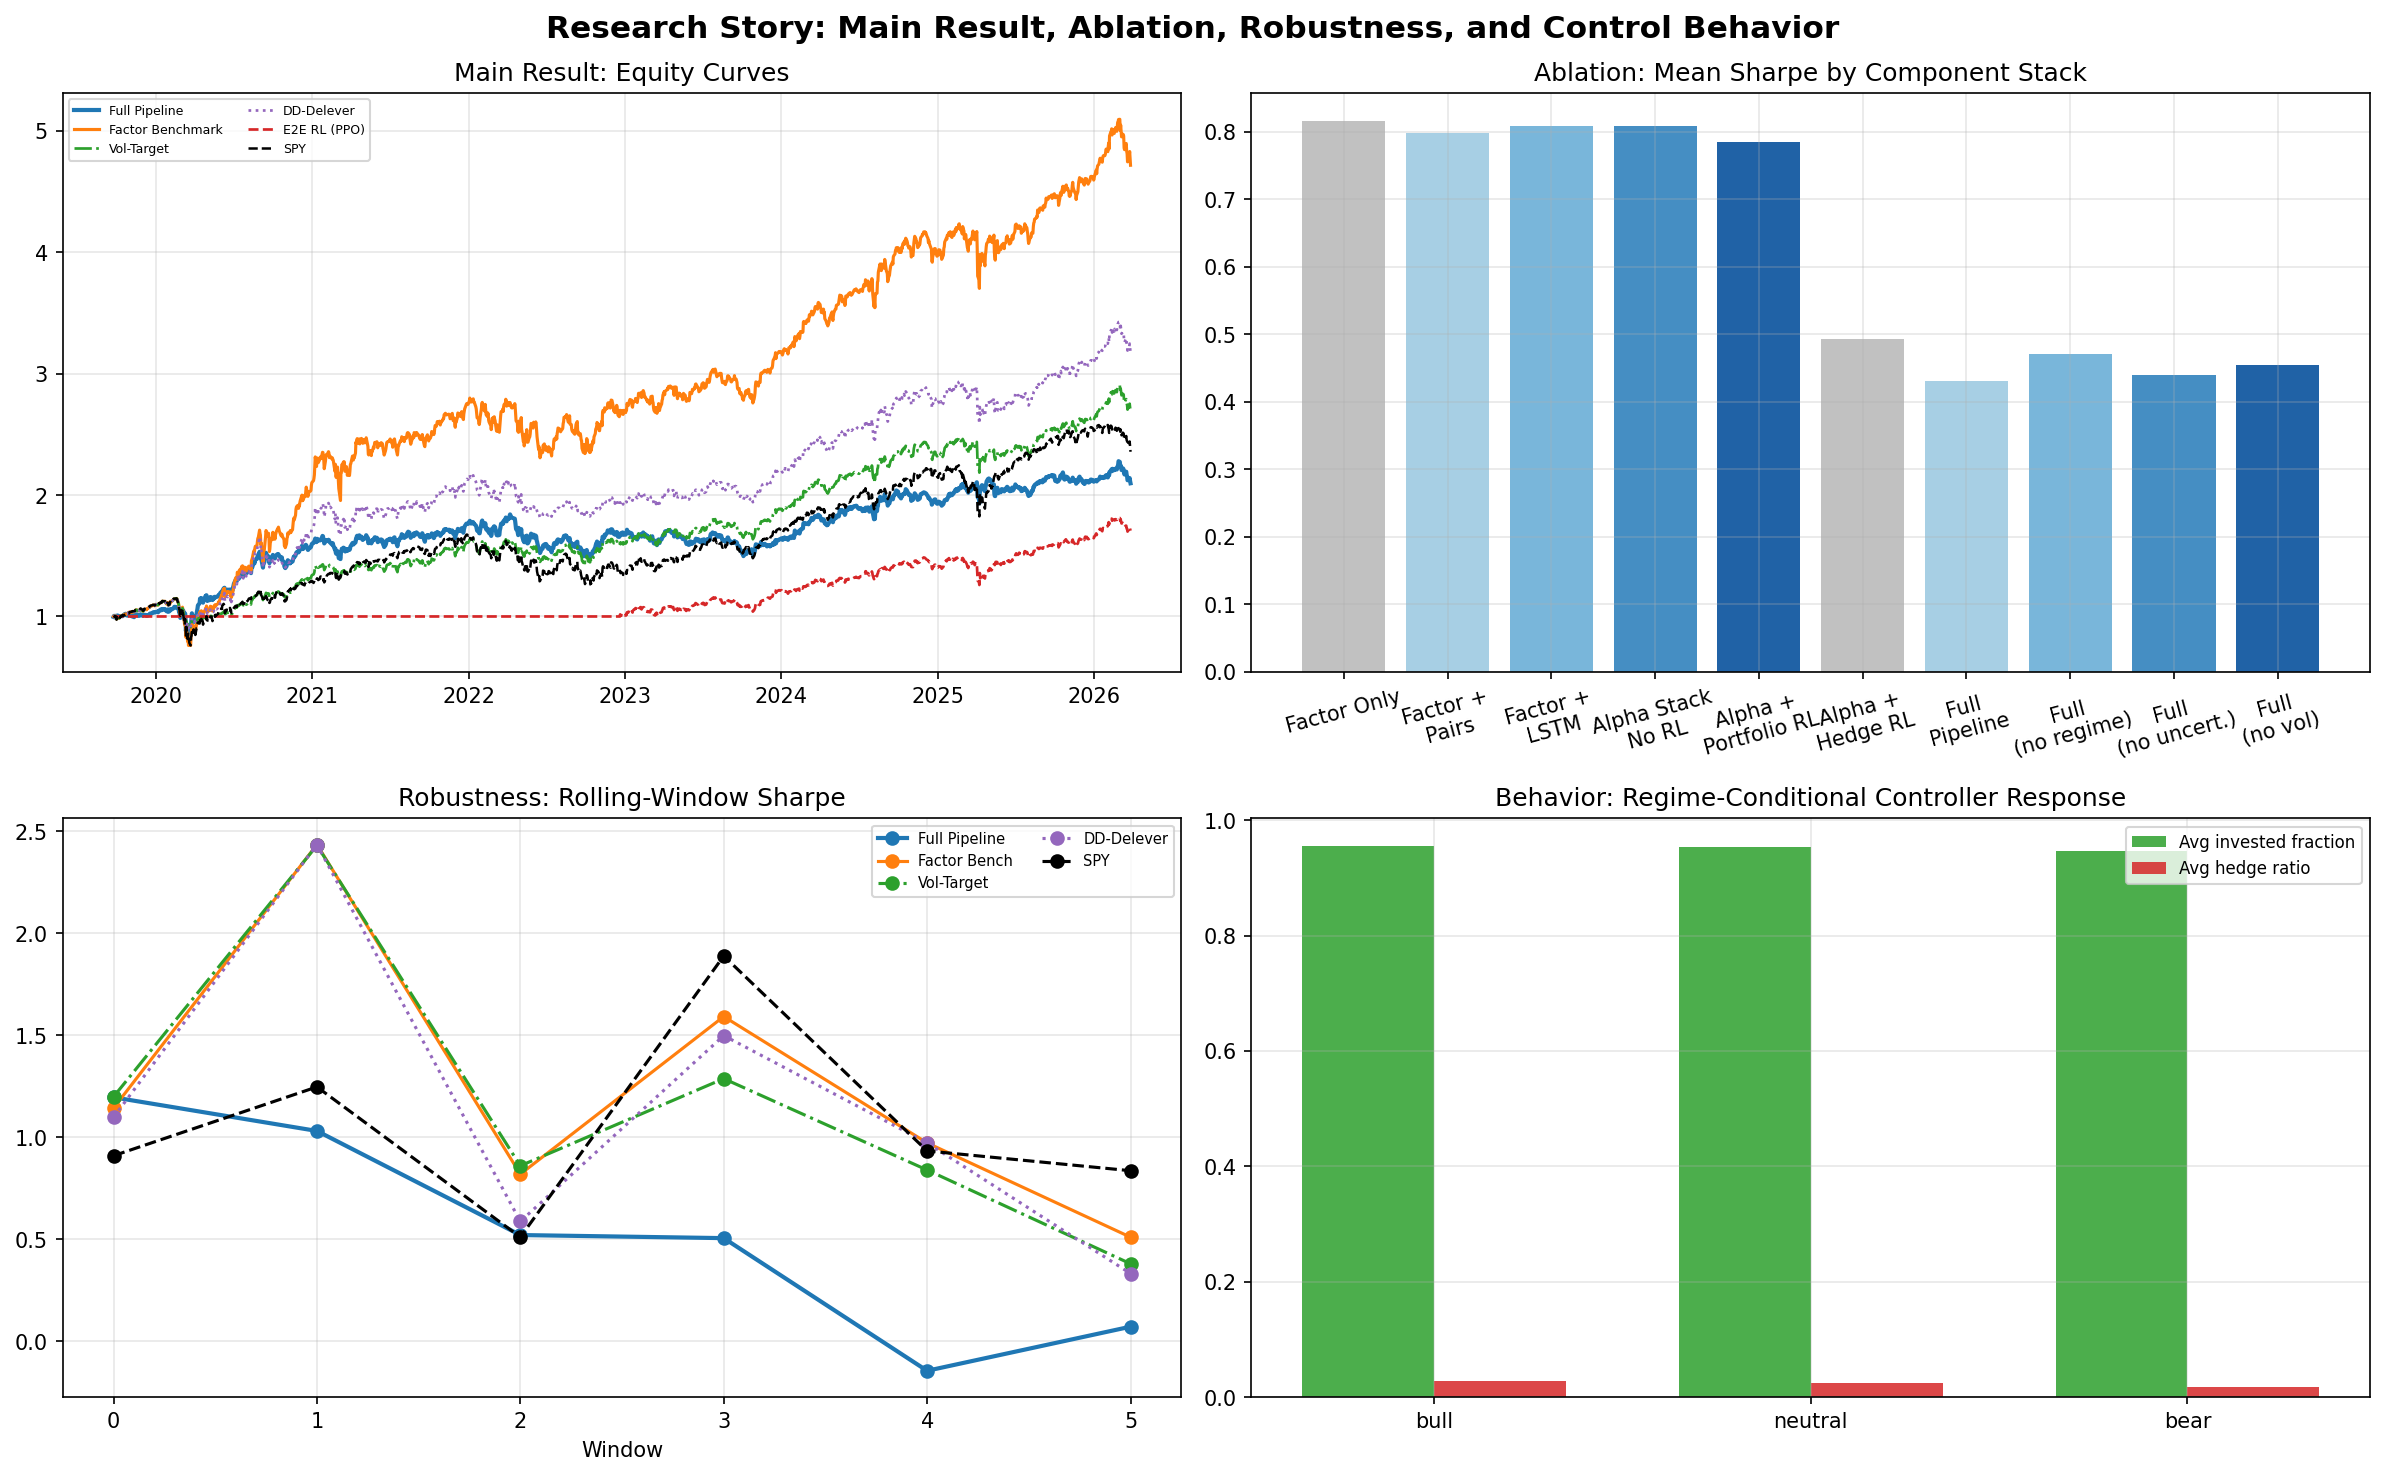
\includegraphics[width=\textwidth]{../../results/20260328_experiments/pipeline_research_eval.png}
\caption{Compact workshop-style summary figure generated by the robustness
engine. The four panels show the main equity-curve result, ablation evidence,
rolling-window robustness, and regime-conditioned controller behavior. The
figure makes clear that the strongest raw-performance outcomes in the archived
bundle come from the factor-only benchmark and the strongest simple overlays,
and that the RL-based variants remain well below those comparators on top-line
metrics.}
\label{fig:research}
\end{figure}
}{
\noindent\textit{Research note.} When the dedicated research runner is executed,
it also emits a compact figure summarizing ablations, rolling-window results,
cost sensitivity, and regime-conditioned policy behavior.
}

\subsection{Ablation Result}

The most important workshop-level question is not whether the full system does
well on one path, but whether the component layering supports the paper's
architectural claim. For that reason the research runner now emits an ablation
summary comparing the factor-only benchmark, the alpha stack without RL, alpha
plus portfolio RL, alpha plus hedge RL, and several reduced-state full-pipeline
variants across multiple split settings.

\begin{table}[t]
\centering
\caption{Ablation summary across train/test split settings.}
\label{tab:ablation_summary}
\begingroup\small
\begin{tabular}{@{} l r r r r r @{}}
\toprule
\textbf{Component} & \textbf{Return} & \textbf{Vol.} & \textbf{Sharpe} & \textbf{Max DD} & \textbf{Calmar} \\
\midrule
Factor-only benchmark & 18.7\% & 18.3\% & 0.82 & $-$26.9\% & 0.72 \\
Factor + pairs        & 18.3\% & 18.3\% & 0.80 & $-$27.1\% & 0.69 \\
Factor + LSTM         & 18.5\% & 18.3\% & 0.81 & $-$27.1\% & 0.70 \\
Alpha stack (no RL)   & 17.9\% & 17.5\% & 0.81 & $-$24.8\% & 0.73 \\
Alpha + portfolio RL  & 16.4\% & 16.1\% & 0.79 & $-$21.7\% & 0.75 \\
Alpha + hedge RL      & 12.4\% & 17.5\% & 0.49 & $-$26.0\% & 0.47 \\
Full pipeline         & 10.7\% & 16.3\% & 0.43 & $-$22.3\% & 0.47 \\
Full (no regime)      & 11.5\% & 16.2\% & 0.47 & $-$22.7\% & 0.50 \\
Full (no uncert.)     & 10.9\% & 16.2\% & 0.44 & $-$23.1\% & 0.46 \\
Full (no vol)         & 11.3\% & 16.4\% & 0.46 & $-$24.5\% & 0.45 \\
\bottomrule
\end{tabular}
\endgroup
\end{table}

\begin{table}[t]
\centering
\caption{Rolling-window robustness summary for the full pipeline.}
\label{tab:robustness_summary}
\begin{tabular}{@{} l r @{}}
\toprule
\textbf{Statistic} & \textbf{Value} \\
\midrule
Rolling windows                                    & 6 \\
Median full-pipeline Sharpe                        & 0.51 \\
Median full-pipeline Calmar                        & 0.83 \\
Median full-pipeline Max DD                        & $-$10.9\% \\
Frac. windows full beats factor-only benchmark on drawdown & 50\% \\
Frac. windows full beats factor-only benchmark on Calmar   & 0\% \\
Frac. windows full beats SPY on Sharpe             & 33\% \\
Frac. windows full beats SPY on Calmar             & 17\% \\
\bottomrule
\end{tabular}
\end{table}

\begin{table}[t]
\centering
\caption{Block-bootstrap significance for full pipeline versus baselines (Sharpe deltas).}
\label{tab:bootstrap_significance}
\begin{tabular}{@{} l r r r @{}}
\toprule
\textbf{Comparison} & \textbf{Delta Sharpe} & \textbf{95\% CI} & \textbf{p-value} \\
\midrule
Full -- SPY                   & -0.05 & [-0.71, 0.45] & 0.830 \\
Full -- Factor-only benchmark & -0.47 & [-0.86, -0.14] & 0.000 \\
Full -- Vol-target            & -0.36 & [-0.78, 0.04] & 0.075 \\
Full -- DD-Delever            & -0.39 & [-0.83, 0.02] & 0.070 \\
Full -- E2E RL (PPO)          & -0.03 & [-1.12, 0.91] & 0.950 \\
\bottomrule
\end{tabular}
\end{table}

The generated ablation table sharpens the story considerably, and more
negatively than before. Averaged across split settings, the factor-only
benchmark remains the strongest pure alpha expression, with mean return 18.7\%
and mean Sharpe 0.82. The pairs and LSTM sleeves add almost no incremental
value on top of that base and slightly worsen average drawdown. The alpha stack
without RL stays close to the factor core on Sharpe, 0.81, while improving mean
maximum drawdown to $-$24.8\%.

Among the RL variants, the best result comes from portfolio RL alone, not from
the hedge sleeve or the full stack. Alpha plus portfolio RL reaches mean Sharpe
0.79, the best mean drawdown in the table at $-$21.7\%, and the highest mean
Calmar among the RL configurations. By contrast, alpha plus hedge RL falls to
mean Sharpe 0.49, and the full pipeline to 0.43.

The additional state features are also not earning their keep in this archived
bundle. Removing regime, uncertainty, or volatility state inputs slightly
improves the full pipeline in every case. This is a stronger pruning result
than the earlier bundle: in the current archived evaluation, neither the hedge
sleeve nor the richer RL state description justifies its added complexity.

\noindent\textit{Implication for RQ3.} Not supported in the intended
direction. The current ablation evidence does not show hedge RL as the main
value driver; if anything, the least-damaging RL contribution comes from
portfolio exposure control alone.

\subsection{Rule-Based and End-to-End Baseline Evidence}

The next layer of evidence asks whether the RL controller is doing something
meaningfully different from simple heuristics. On this archived run, the
volatility-targeting and drawdown-based deleveraging baselines are deliberately
strong comparators: both deliver meaningfully higher return- and Sharpe-based
performance than the full pipeline. The bootstrap and Jobson--Korkie tests point
in the same direction. Relative to the factor-only benchmark, the full
pipeline's Sharpe deficit is clearly negative. Relative to vol-target and
drawdown-based deleveraging, the deficits are borderline to unfavorable,
remaining negative in point estimate and near conventional significance
thresholds.

In the archived sample, RQ2 is not supported. The evidence in this manuscript
does not support the claim that RL adds value over the strongest simple
rule-based overlays on Sharpe or return.

RQ1 receives only weak support at best. The end-to-end PPO baseline earns lower
nominal return than the full pipeline, but slightly higher Sharpe and materially
shallower drawdown. The bootstrap Sharpe delta versus PPO is -0.03 with a wide
confidence interval, and the Jobson--Korkie comparison is likewise far from
significant. The appropriate conclusion is therefore not that modular RL beats
PPO, but that neither RL formulation establishes a convincing edge over
finance-first or rule-based alternatives, while the modular architecture remains
easier to interpret and decompose.

\noindent\textit{Implication for RQ1.} Not strongly supported. The modular
design improves annualized return relative to PPO, but not Sharpe or drawdown,
and the risk-adjusted differences are not statistically decisive.

\noindent\textit{Implication for RQ2.} Not supported in the archived sample:
the strongest simple non-RL overlays outperform the RL controller on return and
Sharpe.

\subsection{Reward-Function Sensitivity}

Reward design affects where the controller lands on the risk-return frontier,
but now only within a fairly narrow band. Across the archived reward-function
ablation, the Sortino-style reward is best, reaching 13.8\% annualized return
and 0.59 Sharpe, while the default differential-Sharpe reward reaches 12.9\%
and 0.53. Mean-variance is the weakest on drawdown-adjusted terms, with maximum
drawdown worsening to $-$25.5\%. Reward choice therefore matters, but it does
not rescue the controller from the broader ranking.

\begin{table}[t]
\centering
\small
\caption{Reward-function ablation for the full pipeline on the archived bundle.}
\label{tab:reward_ablation}
\begin{tabular}{@{} l r r r r @{}}
\toprule
\textbf{Reward} & \textbf{Return} & \textbf{Sharpe} & \textbf{Max DD} & \textbf{Calmar} \\
\midrule
Differential Sharpe & 12.9\% & 0.53 & $-$24.2\% & 0.53 \\
Return              & 13.1\% & 0.54 & $-$23.7\% & 0.55 \\
Sortino             & 13.8\% & 0.59 & $-$23.7\% & 0.58 \\
Mean-Variance       & 13.1\% & 0.55 & $-$25.5\% & 0.51 \\
\bottomrule
\end{tabular}
\end{table}

The archived reward-ablation evidence is therefore specific to the modular full
pipeline. A comparable PPO reward sweep is not treated as primary evidence in
this manuscript because the archived suite did not preserve an equally complete
reward-by-split comparison grid for PPO, and the smaller set of PPO reward runs
is materially noisier because each trial depends on fresh stochastic policy
training.

\noindent\textit{Implication for methodology.} Reward choice matters
substantially for where the controller lands on the risk-return frontier, but it
does not overturn the paper's main qualitative result: reward tuning changes the
controller's operating point within a weak overall band without overturning the
broader qualitative ranking in which the factor-only benchmark and the strongest
simple overlays remain stronger on return- and Sharpe-based comparisons.

\subsection{Robustness Across Windows}

Single-path backtests can be persuasive but are rarely sufficient. The research
runner therefore evaluates the full pipeline across rolling windows and blocked
time-series cross-validation. In the archived run, the rolling-window picture is
materially weaker than in the earlier March 27 bundle: median full-pipeline
Sharpe is 0.51, median Calmar 0.83, and median maximum drawdown $-$10.9\%.
The full pipeline beats SPY on Sharpe in only 33\% of windows and on Calmar in
only 17\% of windows. Relative to the factor-only benchmark, it matches or
improves drawdown in half the windows but never exceeds factor-only on Calmar.

Blocked time-series cross-validation reinforces that instability. Across five
folds, annualized Sharpe ranges from 0.11 to 1.22, with one strong fold and
several much weaker ones. That dispersion suggests substantial regime
dependence rather than a stable control advantage. These windows and folds still
come from one historical sample and should therefore be interpreted as internal
robustness slices rather than independent replications.

The same evidence also sharpens the paper's statistical tone. The bootstrap and
Jobson--Korkie summaries show that the full pipeline is not statistically
distinguishable from SPY or PPO on Sharpe in the archived sample, while its
Sharpe deficit relative to the factor-only benchmark is clearly negative and its
deficits relative to volatility targeting and drawdown-based deleveraging are
borderline to unfavorable. The appropriate claim, then, is not that robustness
is ``won,'' but that the architecture now supports a falsifiable and transparent
protocol for showing when RL does \emph{not} generalize.

\noindent\textit{Implication for the overall claim.} The rolling and
cross-validation evidence do not support a structural edge. At most, they
support occasional drawdown improvement relative to passive exposure.

\IfFileExists{../../results/20260328_experiments/pipeline_rolling_windows.png}{
\begin{figure}[t]
\centering
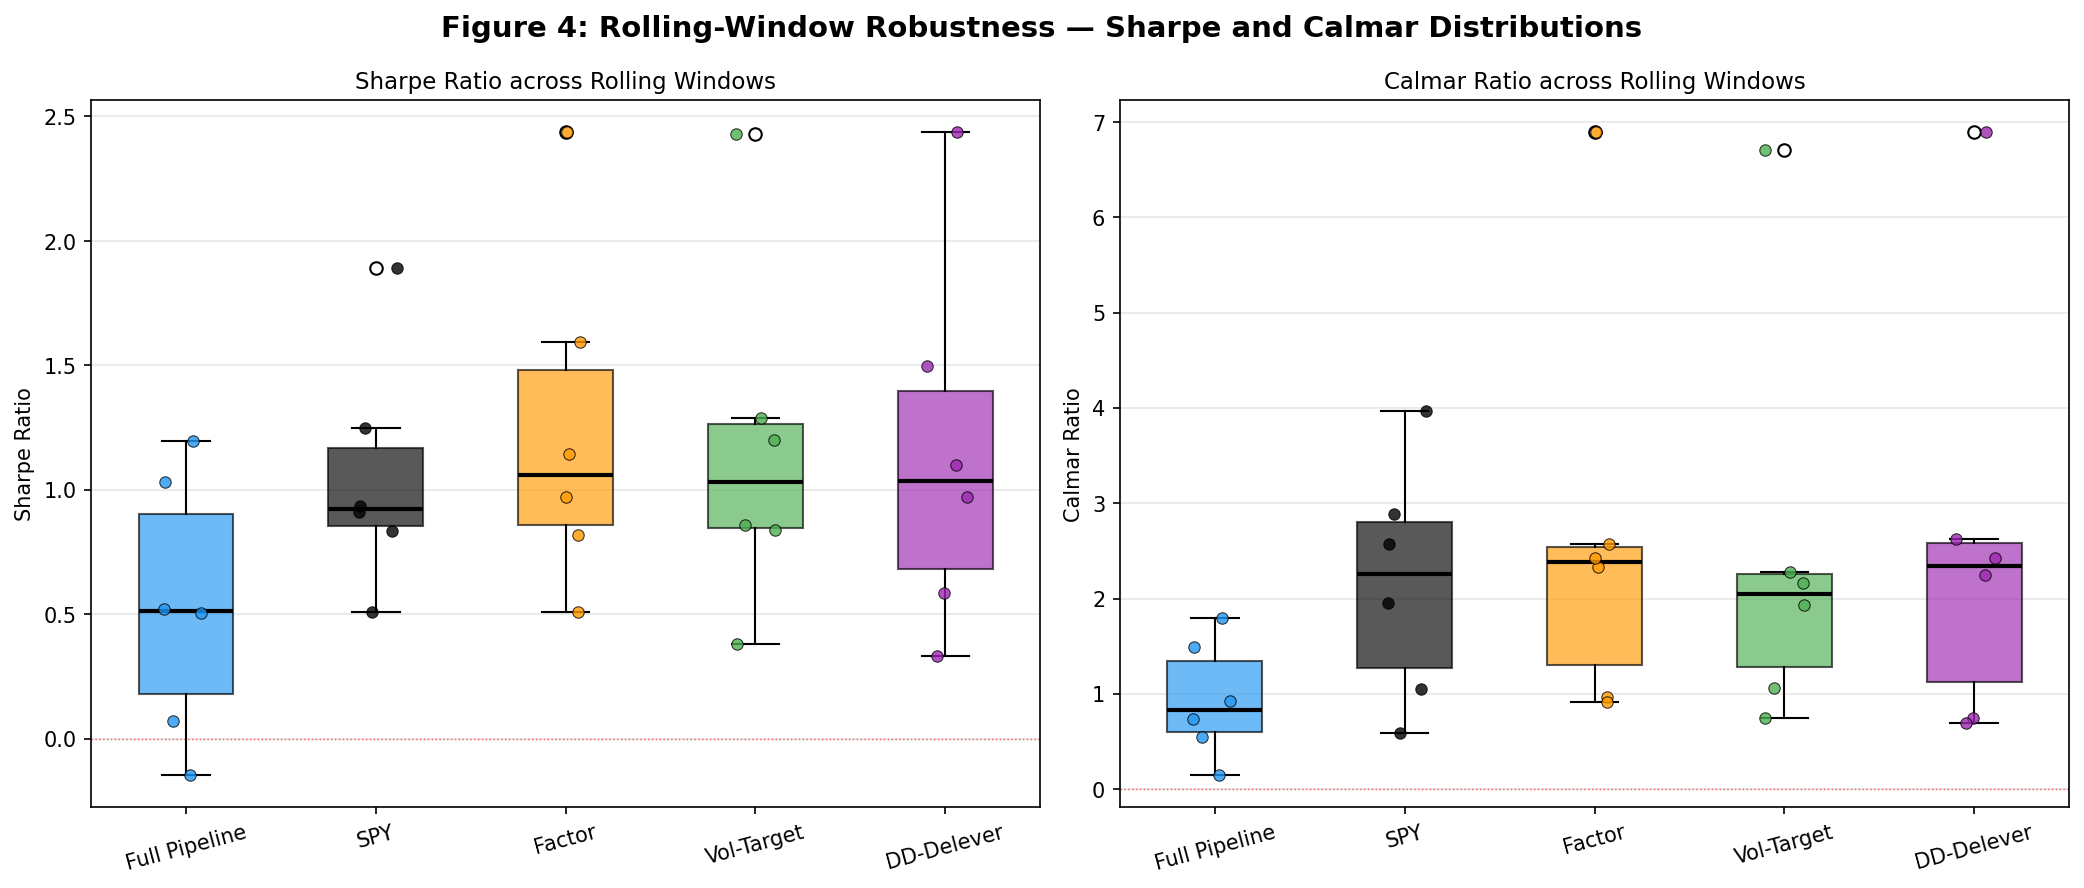
\includegraphics[width=\textwidth]{../../results/20260328_experiments/pipeline_rolling_windows.png}
\caption{Rolling-window robustness from the archived March 28, 2026
experiment bundle. The full pipeline shows mixed performance across windows,
beating SPY on Sharpe in only one-third of slices and never exceeding the
factor-only benchmark on Calmar. These rolling windows are internal robustness
slices from one archived historical sample rather than independent replications.}
\label{fig:rollingwindows}
\end{figure}
}{}

\subsection{Behavioral and Regime Evidence}

The behavioral question is whether the controller is acting like a sequential
decision system. Figure~\ref{fig:research} provides the main summary used in
the paper. The answer in the current archived bundle is only weakly positive.
The controller is not degenerate: it does hold cash, change turnover, and
sometimes select protective-put overlays. But the regime-conditioned summaries
do not show the intended monotone mapping from worse states to lower exposure
and stronger protection.

In the representative full-pipeline split, average portfolio action rises from
about 1.92 in bull states to 2.15 in bear states, while average hedge ratio
falls from roughly 4.9\% to 2.7\%. The dominant hedge type is a protective put
in bull states and no hedge in neutral and bear states. That pattern is hard to
interpret as rational downside control. The more plausible reading is that the
current regime labels, state features, and hedge policy are not yet aligned
tightly enough to produce reliable state-contingent behavior.

\noindent\textit{Implication for RQ3.} Not supported in the intended
behavioral sense. The controller is active, but its hedge and exposure choices
are not yet consistently regime-rational.

\section{Discussion}

The experimental results support three conclusions of methodological importance,
but they are more negative than the previous archived bundle.

First, the data and alpha side of the pipeline is doing most of the credible
work. The factor-only benchmark remains the strongest pure alpha engine, and the
alpha stack without RL stays close on Sharpe while improving drawdown somewhat.
The pairs and LSTM sleeves add little incremental value. In the current
archived evaluation, the strongest evidence is for the factor core and the
constrained non-RL allocator, not for the full RL stack.

Second, the RL layer is currently defensible only in a narrow downside-shaping
sense. In the main split it reduces drawdown relative to SPY, but it does not
beat SPY on return or Sharpe, does not beat the factor-only benchmark or the
best rule-based overlays, and does not produce a clean modular-over-PPO win.
That is still a useful empirical outcome: it shows that the right question is
not ``does RL win?'' but ``what, exactly, does RL change once a finance-first
signal engine is already in place?''

This distinction is central. If the RL layer were treated as a second stock
selector, it would risk duplicating the alpha problem with a less structured
model and less data efficiency. By anchoring the policy to the factor book, the
pipeline preserves interpretability: alpha determines \emph{what} to own, while
RL primarily determines \emph{how much} to own and \emph{what overlay} to carry.
The problem is not that the control formulation is incoherent; it is that the
current controller is not yet adding enough economic value over simpler
alternatives.

What did not work is equally important. RL did not beat the strongest
rule-based overlays on Sharpe or return. The hedge sleeve underperformed the
simpler portfolio-RL-only variant. The richer regime, volatility, and
uncertainty state inputs did not improve the full pipeline relative to stripped-
down versions. The regime-conditioned behavior is not monotone in the intended
direction. These are useful negative results because they narrow where future
improvements should be sought. For a control-layer study, these failures are not
incidental; they are precisely what helps delimit where RL is and is not adding
value.

The practical lesson is therefore more about simplification than expansion.
Further gains are more likely to come from pruning weak sleeves, redesigning the
hedge logic, and validating state features against stronger non-RL baselines
than from adding more controller complexity. True option quotes, cleaner regime
definitions, and less noisy controller objectives may matter more than richer
state spaces by themselves.

\subsection{When Practitioners Should Use This Architecture}

The archived evidence suggests a narrower use case than the paper's original
prototype narrative. This architecture is most defensible as a research or
governance-friendly framework when interpretability and explicit downside
shaping matter more than maximizing Sharpe, and when a credible finance-first
alpha engine already exists underneath the controller.

Simpler alternatives are often sufficient in other settings. If the primary goal
is pure risk-adjusted performance on a daily U.S. equity allocation problem, the
archived bundle suggests that the factor-only benchmark and simple overlays such
as volatility targeting or drawdown-based deleveraging are harder to beat. If
computational budgets are tight, rule-based overlays are also easier to train,
debug, and explain. And if the alpha layer is weak, RL is unlikely to rescue the
system: the controller can reshape risk, but it cannot compensate for the
absence of robust signal quality.

The practical contribution is therefore not ``always use RL.'' It is narrower
still: when RL is used in finance, the current bundle suggests treating it as an
interpretable research instrument for exposure and protection decisions, not yet
as a superior production allocator.

\section{Threats to Validity and Future Work}

The implementation remains research code, and several caveats apply. Macro
inputs are shifted by a configurable lag, but they are not full vintage series
with revision-aware histories. SEC enrichment can be used as a static
cross-sectional prior, but it still does not constitute a true point-in-time
fundamentals database. Transaction costs are more realistic than before, yet
they remain stylized rather than venue-specific. The hedge sleeve in the
archived experiment uses synthetic option-style overlays driven by IV proxies
rather than live option-chain quotes, and the robustness engine still depends
on one underlying historical sample even when it slices that sample in multiple
ways.

Several additional threats deserve explicit acknowledgement. First, the design
has been iterated by observing backtest behavior, which raises the possibility
of researcher degrees of freedom even when each individual change is motivated.
Second, the traded universe is broader than in the earlier prototype but still
narrow relative to institutional equity universes, so the results may depend
partly on the selected names. Third, daily data are appropriate for a medium-
horizon allocation study but cannot validate intraday execution claims. Fourth,
the hedge sleeve is a proxy options implementation rather than a market-priced
options backtest. Finally, the project deliberately leans on free or public data
sources, which improves accessibility but necessarily limits point-in-time
fidelity and market microstructure realism.

A further caveat is benchmark fairness: although the rule-based and PPO
baselines are designed to be strong and informative, their exact specification
still influences comparative conclusions. Because the evaluation suite reports
many metrics and comparator strategies, some apparent wins and losses should
also be interpreted with the usual caution around multiple comparisons.
External validity is also limited: conclusions drawn from a daily U.S.-equity
allocation setting may not transfer unchanged to other asset classes,
frequencies, or market microstructure regimes.

The currently reported robustness summary is still based on only six rolling
windows, five blocked time-series CV folds, and one underlying historical
sample. The workshop interpretation should therefore be that the robustness
engine is now part of the methodology, not that robustness has been exhaustively
established across many independent market environments.

Natural next steps include true filing-date-aware fundamentals, release-vintage
macro datasets, cross-asset regime instruments, and a market-priced hedge sleeve
using live option surfaces rather than IV proxy payoffs. A second important line
of follow-up work is empirical pruning: the LSTM sleeve, the pairs sleeve, and
the richer RL state variables should remain in the architecture only if
ablation continues to show incremental value after further robustness passes.
Finally, while the evaluation engine now includes bootstrap significance and
Jobson--Korkie outputs, future work could push further toward additional
universes, stronger multiple-testing discipline, and deeper validation across
disjoint market regimes.

\section{Conclusion}

This paper shows that a financially grounded hybrid architecture can be modular,
interpretable, and empirically informative even when its RL layer is not a
performance winner. Classical quantitative models remain responsible for alpha
discovery, while reinforcement learning acts as a sequential risk and allocation
controller. The resulting system is not a proof that RL dominates traditional
quant methods. Instead, it is a structured research pipeline whose behavior is
interpretable, testable, and falsifiable.

The main empirical takeaway is narrower and more negative than in the earlier
bundle: in the March 28, 2026 archived evaluation, the modular controller
reduces drawdown relative to SPY in the main split, but it does not beat SPY on
return or Sharpe, does not clearly beat end-to-end PPO, and remains well behind
the factor-only and best rule-based baselines. Equally importantly, the paper
leaves behind a frozen-bundle evaluation protocol that can support future
pruning, hedge redesign, and market-priced options extensions under a consistent
empirical standard. In the reported sample, the evidence supports RL chiefly as
an interpretable risk-shaping overlay and rejects stronger claims of current
economic superiority over finance-first or simple rule-based alternatives.

\appendix

\section{Implementation Snapshot}

\subsection{Archived Experiment Control Ladders}

The March 28, 2026 archived experiment bundle used in the main paper results
relies on the discrete action ladders below. Unlike the earlier bundle, the
reported archived evaluation already includes implied-volatility-conditioned
synthetic hedge-type selection among protective puts, collars, and put spreads.
What remains future work is replacing these proxy payoffs with market-priced
option data.

\begin{center}
\begin{tabular}{lcc}
\toprule
Portfolio action & Invested fraction & Active overlay fraction \\
\midrule
State 0 & 82\% & 5\% \\
State 1 & 90\% & 8\% \\
State 2 & 95\% & 12\% \\
State 3 & 98\% & 16\% \\
State 4 & 100\% & 20\% \\
\bottomrule
\end{tabular}
\end{center}

\begin{center}
\begin{tabular}{lc}
\toprule
Hedge action & Hedge ratio \\
\midrule
State 0 & 0\% \\
State 1 & 3\% \\
State 2 & 8\% \\
State 3 & 15\% \\
\bottomrule
\end{tabular}
\end{center}

\begin{center}
\begin{tabular}{lc}
\toprule
Hedge type action & Overlay type \\
\midrule
Type 0 & Protective put \\
Type 1 & Collar \\
Type 2 & Put spread \\
\bottomrule
\end{tabular}
\end{center}

\subsection{Research Artifacts}

For the archived run discussed in the paper, the research runner writes the
artifacts below into
\path{../../results/20260328_experiments/} alongside the standard paper
outputs:
\begin{enumerate}[leftmargin=1.5em, itemsep=2pt, topsep=4pt]
\item \texttt{research\_metrics.csv}: tabular output for ablation and robustness runs;
\item \texttt{research\_ablation\_summary.csv}: split-aggregated ablation summaries;
\item \texttt{research\_robustness\_summary.csv}: rolling-window medians and benchmark beat fractions;
\item \texttt{research\_regime\_summary.csv}: regime-conditioned action, hedge, turnover, and return summaries;
\item \texttt{research\_rolling\_references.csv}: rolling benchmark metrics for SPY and the factor-only benchmark;
\item \texttt{research\_bootstrap\_cis.csv}: block-bootstrap confidence intervals for key strategy metrics;
\item \texttt{research\_bootstrap\_significance.csv}: pairwise bootstrap deltas and $p$-value summaries versus benchmark strategies;
\item \texttt{research\_jobson\_korkie.csv}: parametric Sharpe-ratio comparison tests;
\item \texttt{research\_ts\_cv.csv}: blocked time-series cross-validation summaries;
\item \texttt{research\_summary.json}: serialized configuration and best-per-suite summaries; and
\item \texttt{research\_paper\_tables.tex} together with
      \texttt{pipeline\_research\_eval.png}: paper-ready summary tables and
      figure.
\end{enumerate}

Together with the feature-availability contract embedded in each backtest run,
these artifacts make it easier to compare results across alternative timing,
cost, and control assumptions without manually reconstructing the experimental
context after the fact.

\subsection{Supplementary Diagnostic Figures}

These figures are diagnostic and illustrative; the primary evidentiary claims
of the paper rest on Tables~\ref{tab:metrics}--\ref{tab:bootstrap_significance}
and Figures~\ref{fig:research} and \ref{fig:rollingwindows}. The appendix
intentionally focuses on figures produced directly by the frozen March 28, 2026
bundle and omits older alpha or execution dashboards that are not tied to the
reported evidence.

\begin{figure}[t]
\centering
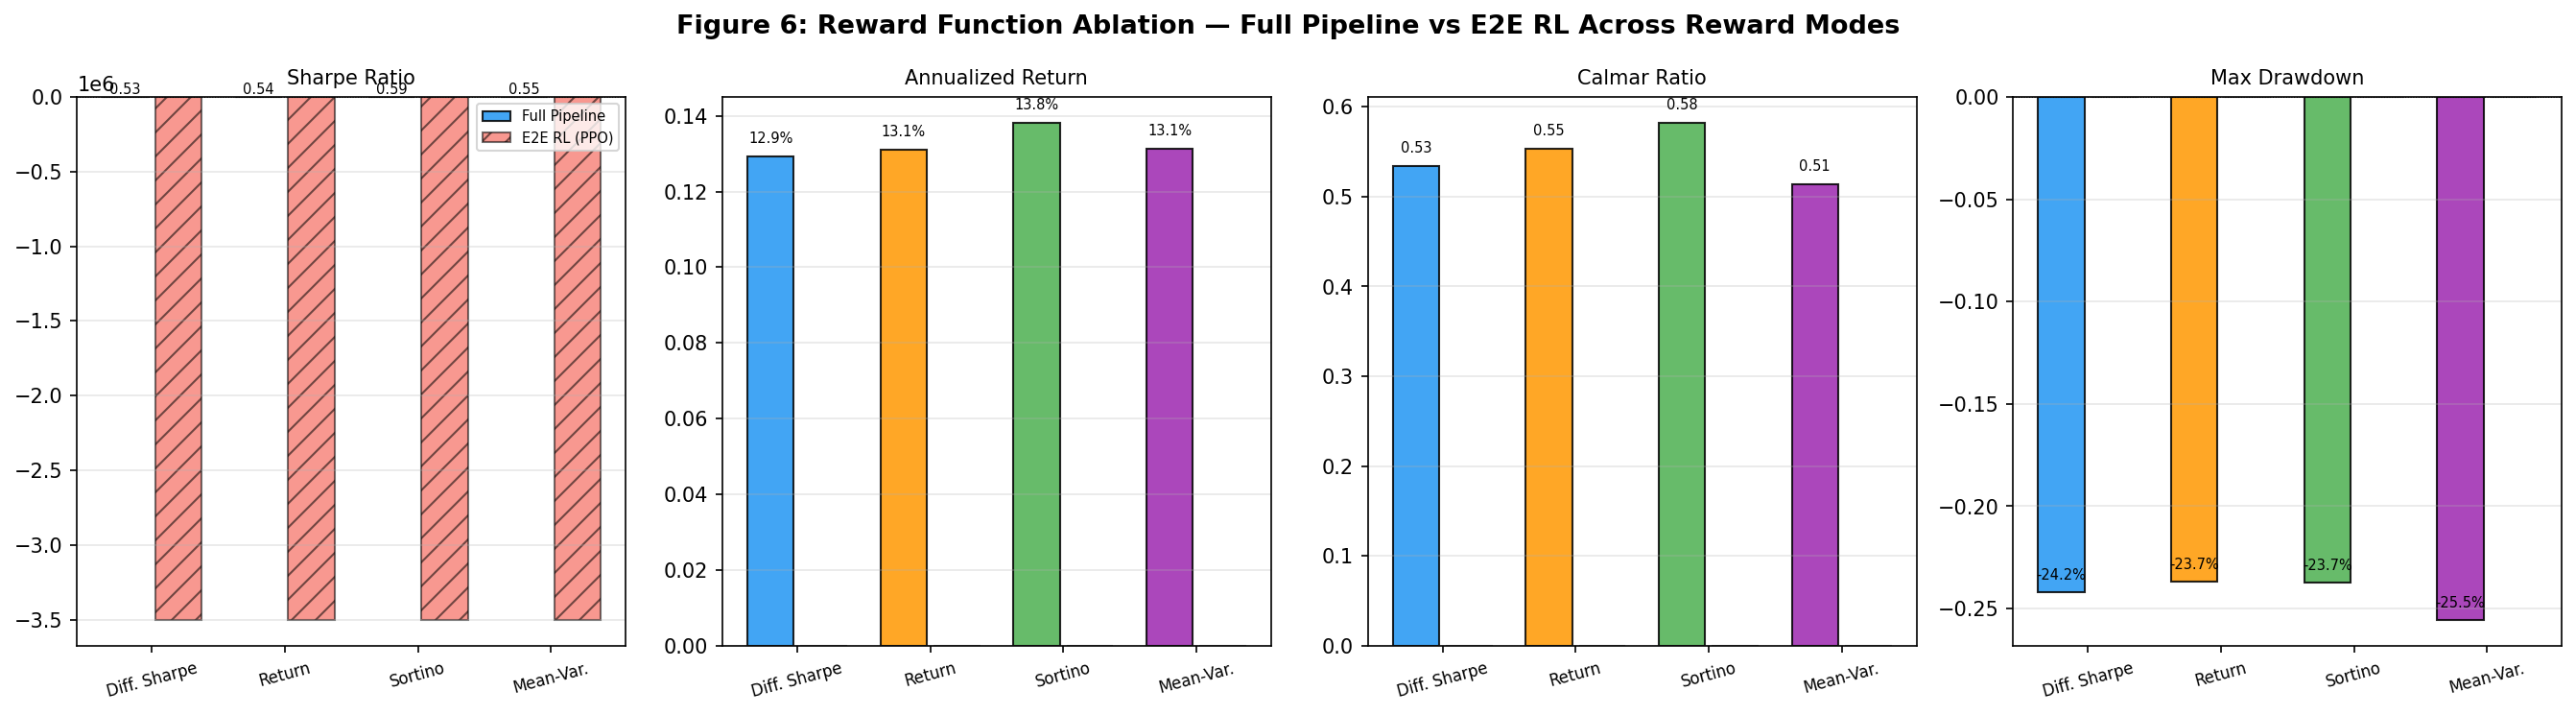
\includegraphics[width=\textwidth]{../../results/20260328_experiments/pipeline_reward_ablation.png}
\caption{Supplementary reward-ablation figure for the archived bundle. Reward
choice moves the full pipeline within a relatively narrow performance band, and
no reward variant changes the broader ranking in which the factor-only benchmark
and the strongest rule-based overlays remain stronger on return- and Sharpe-
based metrics.}
\label{fig:rewardfig}
\end{figure}

\begin{thebibliography}{99}

\bibitem{almgren2000}
R. Almgren and N. Chriss.
\newblock Optimal execution of portfolio transactions.
\newblock \emph{Journal of Risk}, 3(2):5--39, 2000.

\bibitem{buehler2019}
H. Buehler, L. Gonon, J. Teichmann, and B. Wood.
\newblock Deep hedging.
\newblock \emph{Quantitative Finance}, 19(8):1271--1291, 2019.

\bibitem{bollerslev1986}
T. Bollerslev.
\newblock Generalized autoregressive conditional heteroskedasticity.
\newblock \emph{Journal of Econometrics}, 31(3):307--327, 1986.

\bibitem{chen2021}
L. Chen, M. Pelger, and J. Zhu.
\newblock Deep learning in asset pricing.
\newblock \emph{SSRN Working Paper 3350138}, revised 2021.

\bibitem{cong2021}
Y. Cong, B. Deng, X. Bao, and H. Dai.
\newblock AlphaPortfolio: Direct construction through deep reinforcement learning
  and interpretable representation learning.
\newblock \emph{Proceedings of the AAAI Conference on Artificial Intelligence},
  35(6):4831--4839, 2021.

\bibitem{deng2017}
Y. Deng, F. Bao, Y. Kong, Z. Ren, and Q. Dai.
\newblock Deep direct reinforcement learning for financial signal representation
  and trading.
\newblock \emph{IEEE Transactions on Neural Networks and Learning Systems},
  28(3):653--664, 2017.

\bibitem{du2020}
Y. Du, P. N. Kolm, A. Ritter, and T. Wang.
\newblock Deep reinforcement learning for option replication and hedging.
\newblock \emph{The Journal of Financial Data Science}, 2(4):44--59, 2020.

\bibitem{engle1982}
R. F. Engle.
\newblock Autoregressive conditional heteroscedasticity with estimates of the
  variance of United Kingdom inflation.
\newblock \emph{Econometrica}, 50(4):987--1007, 1982.

\bibitem{engle1987}
R. F. Engle and C. W. J. Granger.
\newblock Co-integration and error correction: representation, estimation, and
  testing.
\newblock \emph{Econometrica}, 55(2):251--276, 1987.

\bibitem{fama1993}
E. F. Fama and K. R. French.
\newblock Common risk factors in the returns on stocks and bonds.
\newblock \emph{Journal of Financial Economics}, 33(1):3--56, 1993.

\bibitem{giglio2022}
S. Giglio, D. Xiu, and D. Zhang.
\newblock Machine learning in asset pricing.
\newblock \emph{Annual Review of Financial Economics}, 14:337--368, 2022.

\bibitem{gu2020}
S. Gu, B. Kelly, and D. Xiu.
\newblock Empirical asset pricing via machine learning.
\newblock \emph{Review of Financial Studies}, 33(5):2223--2273, 2020.

\bibitem{hamilton1989}
J. D. Hamilton.
\newblock A new approach to the economic analysis of nonstationary time series
  and the business cycle.
\newblock \emph{Econometrica}, 57(2):357--384, 1989.

\bibitem{jander2025}
J. Jander, H. H. Li, M. Schmid, and T. Pohl.
\newblock Reinforcement learning in finance: From current practice to standards
  and benchmarks.
\newblock \emph{SSRN Working Paper 5703882}, 2025.

\bibitem{jegadeesh1993}
N. Jegadeesh and S. Titman.
\newblock Returns to buying winners and selling losers: implications for stock
  market efficiency.
\newblock \emph{Journal of Finance}, 48(1):65--91, 1993.

\bibitem{jiang2017}
Z. Jiang, D. Xu, and J. Liang.
\newblock A deep reinforcement learning framework for the financial portfolio
  management problem.
\newblock \emph{arXiv preprint arXiv:1706.10059}, 2017.

\bibitem{kolm2019}
P. N. Kolm and G. Ritter.
\newblock Modern perspectives on reinforcement learning in finance.
\newblock \emph{SSRN Working Paper 3449401}, 2019.

\bibitem{kolm2019hedge}
P. N. Kolm and G. Ritter.
\newblock Dynamic replication and hedging: A reinforcement learning approach.
\newblock \emph{The Journal of Financial Data Science}, 1(4):159--171, 2019.

\bibitem{moody2001}
J. Moody and M. Saffell.
\newblock Learning to trade via direct reinforcement.
\newblock \emph{IEEE Transactions on Neural Networks}, 12(4):875--889, 2001.

\bibitem{nevmyvaka2006}
Y. Nevmyvaka, Y. Feng, and M. Kearns.
\newblock Reinforcement learning for optimized trade execution.
\newblock In \emph{Proceedings of the 23rd International Conference on Machine
  Learning}, pages 673--680, 2006.

\bibitem{pacheco2023}
D. Pacheco Aznar.
\newblock Portfolio management: A deep distributional reinforcement learning
  approach.
\newblock \emph{SSRN Working Paper 4522084}, 2023.

\bibitem{sun2023}
S. Sun, M. Qin, W. Zhang, H. Xia, C. Zong, J. Ying, Y. Xie, L. Zhao,
  X. Wang, and B. An.
\newblock TradeMaster: A holistic quantitative trading platform empowered by
  reinforcement learning.
\newblock In \emph{Advances in Neural Information Processing Systems 36:
  Datasets and Benchmarks Track}, 2023.

\bibitem{sutton2018}
R. S. Sutton and A. G. Barto.
\newblock \emph{Reinforcement Learning: An Introduction}.
\newblock MIT Press, Cambridge, MA, second edition, 2018.

\bibitem{zhang2020}
Z. Zhang, S. Zohren, and S. Roberts.
\newblock Deep reinforcement learning for trading.
\newblock \emph{The Journal of Financial Data Science}, 2(2):25--40, 2020.

\end{thebibliography}

\end{document}
